\documentclass[9pt,twocolumn,twoside,lineno]{pnas-new}
% Use the lineno option to display guide line numbers if required.
\usepackage{amssymb}
\usepackage{xcolor}
\usepackage{rotating}
\usepackage{multirow}

\templatetype{pnasresearcharticle} % Choose template 
% {pnasresearcharticle} = Template for a two-column research article
% {pnasmathematics} %= Template for a one-column mathematics article
% {pnasinvited} %= Template for a PNAS invited submission

\title{Protection by vaccines and previous infection against the Omicron variant of SARS-CoV-2}

% Use letters for affiliations, numbers to show equal authorship (if applicable) and to indicate the corresponding author
\author[a,b,1]{Martin \v{S}m\'id}
\author[a,c,d]{Lud\v{e}k Berec} 
\author[e,f]{Ond\v{r}ej M\'ajek}
\author[e,f]{Tom\'a\v{s} Pavl\'{\i}k}
\author[e,f]{Ji\v{r}\'{\i} Jarkovsk\'y}
\author[a,g]{Jakub Weiner}
\author[h]{Lenka P\v{r}ibylov\'a}
\author[i,j]{Tamara Barusov\'{a}}
\author[a,k]{Jan Trnka}

\affil[a]{Centre for Modelling of Biological and Social Processes, Na b\v{r}ehu 497/15, 19000 Praha 9, Czech Republic}
\affil[b]{Czech Academy of Sciences, Institute of Information Theory and Automation, Pod Vod\'arenskou v\v{e}\v{z}\'i 4, 18200 Praha 8, Czech Republic}
\affil[c]{Czech Academy of Sciences, Biology Centre, Institute of Entomology, Department of Ecology, Brani\v{s}ovsk\'a 31, 37005 \v{C}esk\'e Bud\v{e}jovice, Czech Republic}
\affil[d]{Centre for Mathematical Biology, Institute of Mathematics, Faculty of Science,  University of South Bohemia, Brani\v{s}ovsk\'a 1760, 37005 \v{C}esk\'e Bud\'ejovice, Czech Republic}
\affil[e]{Institute of Biostatistics and Analyses, Faculty of Medicine, Masaryk University, Kamenice 126/3, 62500 Brno, Czech Republic}
\affil[f]{Institute of Health Information and Statistics of the Czech Republic, Palack\'eho n\'am\v{e}st\'i 4, 12801 Praha 2, Czech Republic}
\affil[g]{Siesta Labs, Konopi\v{s}\v{t}sk\'a 739/16, 10000 Praha 10, Czech Republic}
\affil[h]{Department of Mathematics and Statistics, Faculty of Science, Masaryk University, 61137 Kotl\'a\v{r}sk\'a 2, Brno, Czech Republic}
\affil[i]{First Faculty of Medicine, Charles University, Kate\v{r}inská 32, 12108 Praha 2, Czech Republic}
\affil[j]{Czech Academy of Sciences, Institute of Computer Science, Department of Statistical Modelling, Pod Vodárenskou věží 2, 18207 Praha 8, Czech Republic}
\affil[k]{Department of Biochemistry, Cell and Molecular Biology, Third Faculty of Medicine, Charles University, Ruská 87, 10000 Praha 10, Czech Republic}

% Please give the surname of the lead author for the running footer
\leadauthor{\v{S}m\'id} 

% Please add a significance statement to explain the relevance of your work
\significancestatement{A nation-wide study shows that the protection of a previous infection or vaccination is lower against Omicron compared to Delta variant of SARS-CoV-2 and further declines with time. A booster dose or a combination of post-infection immunity with a vaccine conferred significant benefit to individuals in the Omicron wave in the Czech Republic, which further strengthens the importance of vaccination as an effective public health measure.
%Authors must submit a 120-word maximum statement about the significance of their research paper written at a level understandable to an undergraduate educated scientist outside their field of speciality. The primary goal of the significance statement is to explain the relevance of the work in broad context to a broad readership. The significance statement appears in the paper itself and is required for all research papers.
}

% Please include corresponding author, author contribution and author declaration information
\authorcontributions{ LB, M\v{S}, JT and LP conceived this study. JJ, OM, JW, and TB prepared and checked the data, TP provided the methodological expertise, JW and M\v{S} conducted the analyses. LB and JT wrote the first draft of the manuscript. All authors contributed to writing the manuscript and interpreting the results. All authors approved the final version and had final responsibility for the decision to submit for publication.}
\authordeclaration{All authors declare no competing interests.}
%\equalauthors{\textsuperscript{1}A.O.(Author One) contributed equally to this work with A.T. (Author Two) (remove if not applicable).}
\correspondingauthor{\textsuperscript{1}To whom correspondence should be addressed. E-mail: smid@utia.cas.cz}

% At least three keywords are required at submission. Please provide three to five keywords, separated by the pipe symbol.
\keywords{covid-19 $|$ post-infection immunity $|$ vaccine effectiveness $|$ SARS-CoV-2 $|$ Omicron variant $|$ hospitalization} 

\begin{abstract}
The Omicron variant of the SARS-CoV-2 virus carries mutations, which enable it to evade immunity conferred by vaccines and previous infections.
We used a Cox proportional hazards model and a logistic regression model on individual-level data on all laboratory-confirmed SARS-CoV-2 infections in the Czech Republic to estimate the relative risk of infection, hospitalization, including severe states, for Delta and Omicron variants, adjusting for sex, age, previous infection, vaccine type and vaccination status.
A recent (<2 months) two-dose vaccination reached VE 43\% (95\% CI: 42-44) against infection by Omicron compared to 73\% (95\% CI: 72-74) against Delta. A recent booster increased VE to 56\% (95\% CI: 55-56) against Omicron infection compared to 90\% (95\% CI: 90-91) for Delta. The VE against Omicron hospitalization of a recent two-dose vaccination was 45\% (95\% CI: 29-57), with a recent booster 87\% (95\% CI: 84-88). The VE against the need for oxygen therapy due to Omicron was 57\% (95\% CI: 32-72) for recent vaccination, 90\% (95\% CI: 87-92) for a recent booster. Post-infection protection against Omicron hospitalization declined from 68\% (95\% CI: 68-69) at <6 months to 13\% (95\% CI: 11-14) at >6 months after a previous infection. A recent combination of a previous infection and vaccination was more protective then either alone with a slight benefit from a vaccination preceding an infection. Once infected, the OR for Omicron relative to Delta was 0.36 (95\% CI: 0.34-0.38) for hospitalization, 0.24 (95\% CI: 0.22-0.26) for oxygen therapy, and 0.24 (95\% CI: 0.21-0.28) for ICU admission.
\end{abstract}

\dates{This manuscript was compiled on \today}
\doi{\url{www.pnas.org/cgi/doi/10.1073/pnas.XXXXXXXXXX}}

\def\nocase{no case}


\begin{document}

\maketitle
\thispagestyle{firststyle}
\ifthenelse{\boolean{shortarticle}}{\ifthenelse{\boolean{singlecolumn}}{\abscontentformatted}{\abscontent}}{}


\dropcap{T}he B.1.1.529 (Omicron) variant of SARS-CoV-2 was first detected in South Africa in November 2021, immediately designated a variant of concern by the WHO \citep{who2021omicron} and  thereafter seen quickly to spread throughout most of the world. This rapid spread was at least in part brought about by a degree of immune evasion due to a large number of mutations in the viral S-protein, which led to changes in epitopes recognised by antibodies elicited by vaccination or previous infection \citep{mccallum2022}. Together with non-pharmacological interventions such as face masks, distancing, ventilation of interior spaces testing and isolating, vaccination is among the most effective means of individual and collective protection from the impacts of the pandemic. The immune evasion by the Omicron variant thus caused concern and led to a lot of interest in both laboratory and real-life epidemiological data that could accurately measure this phenomenon.
\label{sec1}


Since December 27, 2020 the inhabitants of the Czech Republic have been receiving covid-19 vaccines with the largest number vaccinated with the mRNA vaccine Comirnaty (BNT162b2, Pfizer/BioNTech), followed by Spikevax (mRNA-1273, Moderna), and the adenovirus-based vector vaccines Vaxzevria (ChAdOx1 nCoV-19, AstraZeneca) and Janssen Covid-19 Vaccine (Ad26.CoV2.S, Johnson\&Johnson, further abbreviated as Janssen) \citep{mzcr}. By February 13, 2022, the end of our study period, 68\% of the population had a complete vaccination and 39\% received a booster dose  \citep{mzcr} 

The first case of the Omicron variant in the Czech Republic was detected at the end of November 2021, its proportion of recorded cases rapidly rose and by January 10, 2022 it became the dominant variant , see Figure \ref{fig:discrim}. An increasing number of infections among fully vaccinated and re-infections indeed suggests that immune evasion poses a significant risk to further covid-19 development \citep{mzcr}. 

In this study, we estimate how the protection due to vaccination or previous SARS-CoV-2 infection against covid-19 infection, hospital admission, oxygen therapy and ICU admission varies in relation to the virus variant and time elapsed for the whole population of the Czech Republic.

\begin{SCfigure*}[\sidecaptionrelwidth][t]
\centering
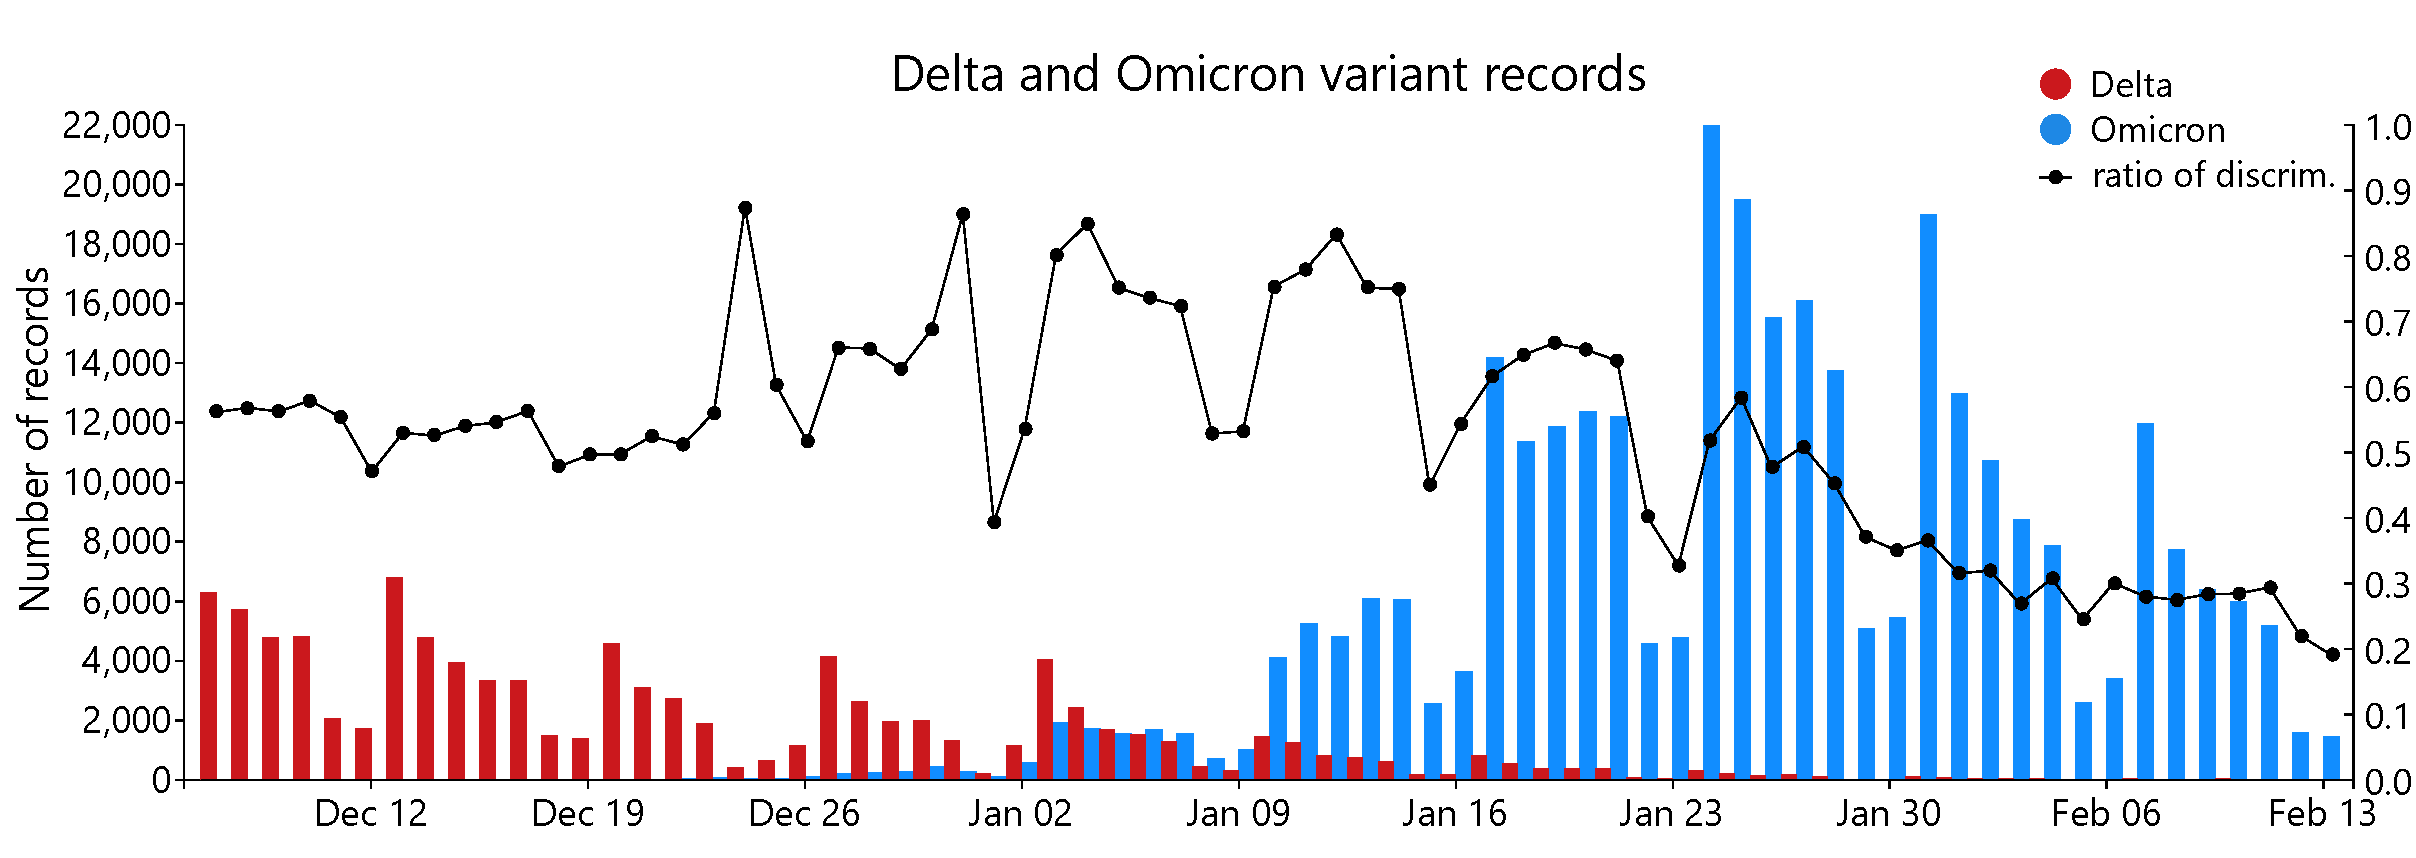
\includegraphics[width=0.85\textwidth]{fig1.pdf}
\caption{Number of recorded cases with assigned Delta (red) and Omicron (blue) variant and the proportion of PCR positive tests (black) tested for viral variants using multiplex PCR.}
\label{fig:discrim}
\end{SCfigure*}

\section*{Methods}
\label{sec2}

\subsection*{Study population and data sources}

The analyses are based on data from the Czech National Information System of Infectious Diseases (ISID), which includes records of all individuals tested positive for SARS-CoV-2 in the Czech Republic since the beginning of covid-19 pandemic, including children \citep{komenda2020}. This database is overseen by the Czech Ministry of Health and operated by the Institute of Health Information and Statistics of the Czech Republic. Data are routinely collected in compliance with Czech legal regulations (Act on the Protection of Public Health). The Director of the Institute of Health Information and Statistics of the Czech Republic has granted an ethical approval of the retrospective analyses presented in this paper.

The ISID database collects demographic data (age, sex and region of residence), dates of vaccination, including the vaccine types for each dose, and dates of infection and potential reinfection, hospitalization including treatment type and the date of potential death with covid-19. Approximately half of data recorded in the study period include information on whether the infection is caused by the Omicron, Delta, some other variant, or that a variant discrimination was not performed. The information on the Omicron variant is based on results of multiplex PCR or viral genome sequencing, which are available only for a subset of all PCR-positive cases. The identification of Delta, Omicron, or other variant was computed using definition of viral S-protein mutations according to ECDC \citep{ECDC_var_concern}; the algorithm was tailored to multiplex PCR kits used in the Czech Republic in collaboration with the National Institute of Public Health and the National Reference Laboratory \citep{SZU_zprava}. Additional information on deaths from any cause come from the Death Certificate System; these data are used for censoring purposes only.

\subsection*{Study endpoints}

We studied four types of events: (i) SARS-CoV-2 infection defined as a PCR-confirmed positive test of any type of sample regardless of the presence of symptoms, (ii) hospital admission of a person, who tested positive on a PCR test, within two weeks after the confirmed infection or earlier, (iii) use of any type of oxygen therapy (nasal oxygen, noninvasive ventilation, invasive mechanical ventilation, high-flow nasal oxygen, and extracorporeal membrane oxygenation) and (iv) admission to ICU during the hospitalization. All events were related to the date of infection report.

We examined events during the two month period from December 7, 2021 to February 13, 2022 during which Delta and Omicron switched dominance in the Czech Republic (Fig. \ref{fig:discrim}). 

\subsection*{Statistical analysis}
A Cox regression with time-varying covariates was applied to estimate hazard ratios (HRs) for the outcomes of interest separately for each viral variant. In these analyses the infections by the variant other than the examined one and the infections lacking variant assignment were censored at the time of infection. Analogously to \citep{tartof2021effectiveness} we used calendar time instead of time from event occurrence as the time scale. Thus the time course of individual cases was modelled by means of ``switching'' dummy variables, corresponding to the development of the immune status after vaccination or past infection in 61-day periods for vaccination and 121-day periods for the time from the last infection.

The protection provided by vaccine (vaccine effectiveness) or previous infection is calculated by comparing hazards of the vaccinated and/or immunized individuals to those of the  ``control group'' -- those who have not been vaccinated and infected so far and subtracted from 1 using the equation:
\begin{equation}
Protection\, (\mbox{VE}) = 1 -  \frac{\mathrm{Hazard_{protected}}}{\mathrm{Hazard_{unprotected}}}
\label{eq1}
\end{equation}

Further we examine the post-infection immunity by estimating hazard ratios of infection of previously unvaccinated individual in relation to time elapsed from the infection. By using calendar time we were able automatically to incorporate the changing conditions of the epidemic, including non-pharmacological measures, seasonal effects, and the  virus variant, as all of these phenomena can be included in the underlying baseline hazard function. 

To examine the probabilities of hospitalization, oxygen therapy and ICU admission for an infected individual we use the logistic regression with the event of interest as the outcome and with all infections with an assigned viral variant as the data. By means of the dummy corresponding to the virus variant we compare the probabilities of the outcome for both the variants. Post-infection and post-vaccination status, age and sex are used as control variables. To estimate the amount of protection provided by the vaccination and/or past infection we run the logistic regression separately for infections by the two variants. %(ale nevím, jestli to Luděk nakonec použije)

 
All calculations were performed using the R software (package \verb|survival|). The algorithm used to transform data from the database into the package command inputs was coded in C++. See Supplementary material 1 for details. 


\section*{Results}
\label{sec3}

\subsection*{Protection against infection}

First we looked at the protection conferred by vaccination or a previous infection against a new infection, since the protection against infection represents the potential to protect others at risk in the population. For vaccination and the Omicron variant the protection reached 43\% (95\% CI 42-44) shortly after completing the full vaccination scheme, falling to 9\% (95\% CI 8-10) after more than two months. This protection increased to 56\% (95\% CI 55-56) shortly after receiving a booster dose, followed by a decline to 21\% (95\% CI 19-23) after more than two months. These numbers strongly contrast with the protection against the Delta variant, which was consistently higher at 73\% (95\% CI 72-74), 57\% (95\% CI 56-58), 90\% (95\% CI 90-91) and 82\% (95\% CI 79-84), respectively. Similar degrees of protection against infection are conferred also by the post-infection immunity: 68\% (95\% CI 68-69) shortly after infection (2-6 months, a positive test during the first two months after an infection is not considered a reinfection by definition) and 13\% (95\% CI 11-14) after six months for Omicron, versus 95\% (95\% CI 94-96) shortly after infection and 83\% (95\% CI 82-84) after six months for Delta (Figure \ref{figIalone}). Based on the past prevalence of viral variants it can be expected that the infections older than 6 months were mostly due to the original Wuhan, D614G and Alpha variants, while the more recent ones were predominantly due to Delta. As we show in the Supplementary material 2, Sections 11 and 12, explicit accounting for the vaccine type Comirnaty (BNT162b2, Pfizer/BioNTech) and Spikevax (mRNA-201273, Moderna) gave values of effectiveness comparable with the analyses of pooled data reported here in the main text.   

\begin{figure}[h]
\centering
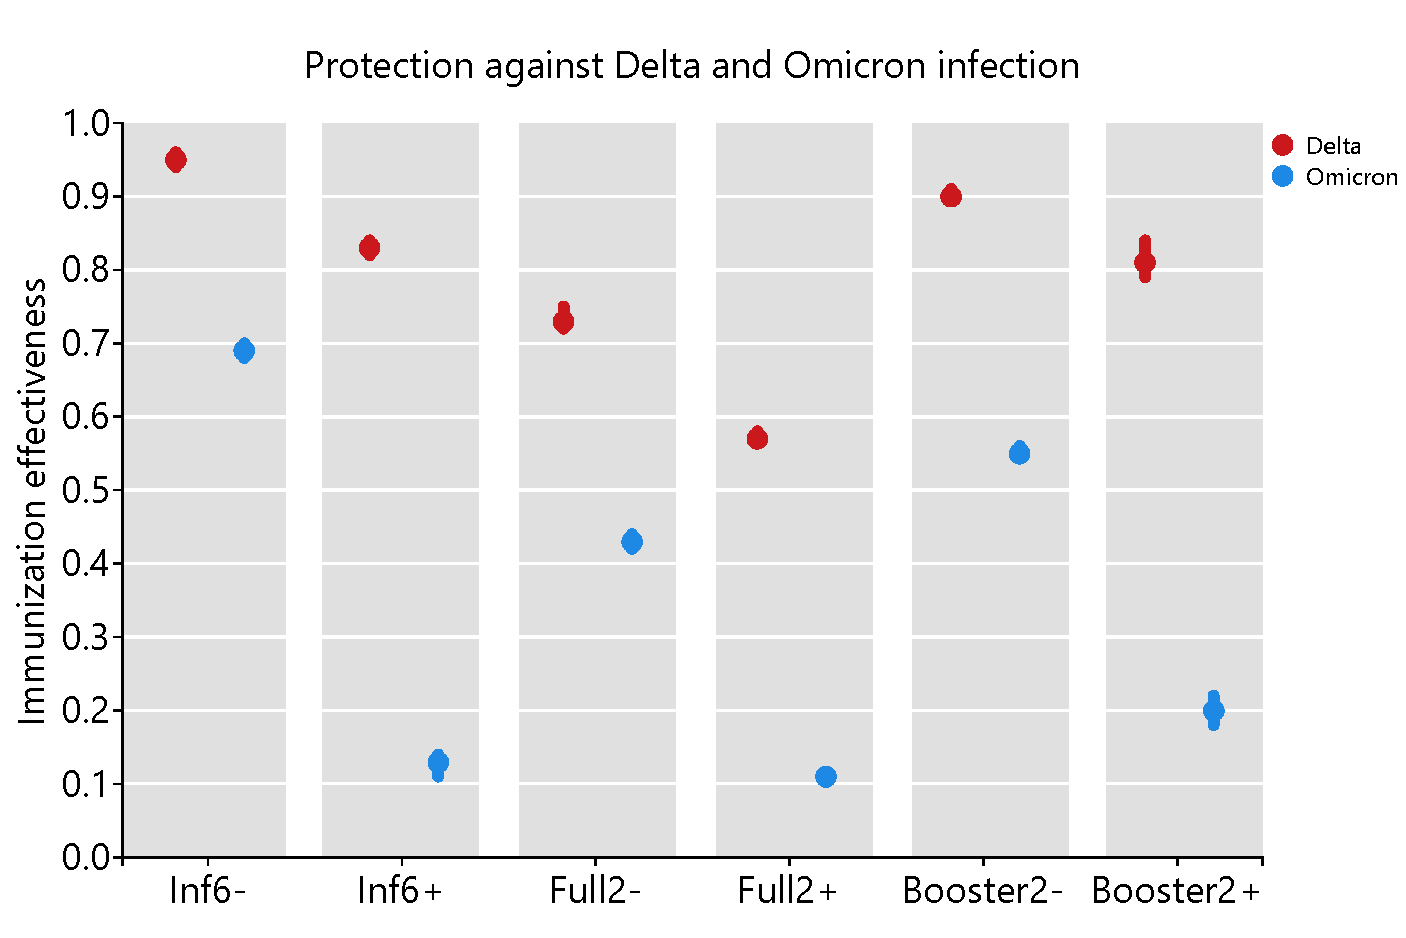
\includegraphics[width=\linewidth]{fig2.pdf}
\caption{Protection provided by vaccination or previous infection against infection by the Omicron and Delta variants of the SARS-CoV-2 virus. Inf6-, previous infection <6 months ago; Inf6+, previous infection >6 months ago; Full2-, complete vaccination <2 months ago;  Full2+, complete vaccination >2 months ago; Booster2-, booster dose <2 months ago; Booster2+, booster dose >2 months ago. Shown are point estimates of protection with 95\% CI.}
\label{figIalone}
\end{figure}

We had enough data to examine all the combinations in which a previous infection preceded vaccination. As expected, protection declined with time elapsed from the previous infection or vaccination (Tables \ref{tabIOinteractions} and \ref{tabIDinteractions}). For the Delta variant, any combination provided $\geq 95\%$ protection against infection (Table \ref{tabIDinteractions}). This protection remained quite high also for Omicron when the previous infection was recent, falling to lower values for an older previous infection, but even then the protection was significantly higher than for a vaccination or previous infection alone (Table \ref{tabIOinteractions}). We also analysed cases, where a vaccination preceded a previous infection, and conclude that when the protection is high (against Delta) then the order of events does not matter (see description of Tab. \ref{tabIDinteractions}). However, when protection is lower (against Omicron), the situation when a previous infection followed a vaccination appeared to provide a higher protection than the inverse sequence (see the caption of Tab. \ref{tabIOinteractions}). The protection provided by Full 2+/Inf 6- combination was 89\% (88-91) as compared to 86\% (95\% CI 85-88) for Inf 6-/Full 2+.

\newcolumntype{L}[1]{>{\raggedright\let\newline\\\arraybackslash\hspace{0pt}}m{#1}}
\newcolumntype{C}[1]{>{\centering\let\newline\\\arraybackslash\hspace{0pt}}m{#1}}
\newcolumntype{R}[1]{>{\raggedleft\let\newline\\\arraybackslash\hspace{0pt}}m{#1}}

\begin{table}[!ht]
\caption{Protection due to various combinations of past infection preceding vaccination  {\it against infection} for the {\it Omicron} variant of the SARS-CoV-2 virus.  Infection in recent 6 months is denoted as Inf 6- and older Inf 6+, completed vaccination scheme is denoted Full 2- for completion in recent 2 months and Full 2+ for older completion, analogously for booster. In parentheses, 95\% confidence intervals (CI) are given. The inverse immunisation order had a higher effect: more than 2 months old full vaccination followed by infection in recent 6 months had 89\% (88-91\%) for full vaccination.}
\label{tabIOinteractions}
\centering
\begin{tabular}{|C{.1\linewidth}|C{.16\linewidth}|C{.16\linewidth}|C{.16\linewidth}|C{.16\linewidth}|}
\hline
\cellcolor{gray!20}$o$ {\it inf}&\cellcolor{gray!20}Booster 2- & \cellcolor{gray!20}Full 2-&\cellcolor{gray!20}Booster 2+& \cellcolor{gray!20}Full 2+\\
\hline
\cellcolor{gray!20}&92\%&82\%&82\%&86\% \\
 \multirow{-2}{*}{\cellcolor{gray!20}Inf 6-}&(89-94\%)& (75-87\%)&(72-89\%)&(85-88\%)\\
\hline
\cellcolor{gray!20}&74\%&77\%&48\%&45\%\\
 \multirow{-2}{*}{\cellcolor{gray!20}Inf 6+}&(73-75\%)&  (76-78\%) &(45-52\%)&(44-46\%)\\
\hline 
\end{tabular}
\end{table}

\begin{table}[!ht]
\caption{Protection due to various combinations of past infection preceding vaccination {\it against infection} for the {\it Delta} variant of the SARS-CoV-2 virus, 95\% confidence intervals (CI) in parentheses. The inverse immunisation order: more than 2 months old full vaccination followed by infection in recent 6 months had protection 96\% (90-98\%) for full vaccination.}
\label{tabIDinteractions}
\centering
\begin{tabular}{|C{.1\linewidth}|C{.16\linewidth}|C{.16\linewidth}|C{.16\linewidth}|C{.16\linewidth}|}
\hline
\cellcolor{gray!20}$\delta$ {\it inf}&\cellcolor{gray!20}Booster 2-&\cellcolor{gray!20}Full 2-&\cellcolor{gray!20}Booster 2+ &\cellcolor{gray!20}Full 2+\\
\hline
\cellcolor{gray!20}&95\%&100\%&100\%&97\%\\
 \multirow{-2}{*}{\cellcolor{gray!20} Inf 6-}&(66-99\%)& \nocase&\nocase&(94-98\%)\\
\hline
\cellcolor{gray!20}&98\%&98\%&94\%&96\%\\ \multirow{-2}{*}{\cellcolor{gray!20}Inf 6+}&(98-99\%)&(97-98\%)&(89-97\%)&(95-96\%)\\
\hline
\end{tabular}
\end{table}

These levels of protection against infection provided by vaccination or previous infection were estimated from the complete set of data. A finer grained analysis of temporal dynamics of immunity waning after a previous infection was then conducted specifically for individuals that were previously infected but remained non-vaccinated. For Omicron, the protection was estimated as 69\% (95\% CI 68-69) for 2-6 months after previous infection,  48\% (95\% CI 46-50) for 7-10 months, 34\% (95\% CI 33-35) for 11-14 months, and 17\% (95\% CI 15-18) for 14 and more months after previous infection. For Delta, on the contrary, these numbers were 93\% (95\% CI 91-94), 91\% (95\% CI 90-92), 86\% (95\% CI 85-86), and 79\% (95\% CI 77-81), respectively.

\subsection*{Protection against hospitalization}

Qualitatively similar pattern yet quantitatively consistently higher protection is seen against hospitalization (Tables \ref{tabHalone}), a need for oxygen therapy (Tables \ref{tabOalone}), and a need for intensive care (Tables \ref{tabUalone}). 
For example, a recent booster dose provides 87\% protection against hospitalization, 90\% against a need of oxygen therapy, and 84\% against a need of intensive care for the Omicron variant. Moreover, all combinations of previous infection and vaccination present in our data appear to provide nearly complete protection against Omicron as regards hospitalization (Tables \ref{tabHOinteractions} and \ref{tabHDinteractions}) as well as against need of oxygen therapy or intensive care (no cases have been observed for such situations).

\begin{table}[!ht]
\caption{Vaccine effectiveness and protection provided by post-infection immunity {\it against hospitalization}, for the Omicron and Delta variants of the SARS-CoV-2 virus, 95\% confidence intervals (CI) in parentheses.}
\label{tabHalone}
\centering
\begin{tabular}{|l|c|c|}
\hline
\cellcolor{gray!20}Effect ag. {\it Hosp.} & \cellcolor{gray!20} Omicron & \cellcolor{gray!20} Delta \\
\hline
Full 2-&45\% (29-57\%)&75\% (68-80\%)\\
\cellcolor{gray!10}Full 2+&\cellcolor{gray!10}29\% (21-37\%) &\cellcolor{gray!10}79\% (78-81\%)\\
Booster 2-&87\% (84-88\%)&98\% (97-98\%)\\
\cellcolor{gray!10}Booster 2+&\cellcolor{gray!10}79\% (75-83\%)&\cellcolor{gray!10}97\% (95-98\%)\\
Inf 6-& 
%73\% (55-84\%)
87\% (73-94\%)
&100\% (\nocase)\\
\cellcolor{gray!10}Inf 6+&\cellcolor{gray!10}
%66\% (54-75\%) 
92\% (86-96\%) 
&\cellcolor{gray!10}95\% (93-96\%)\\
\hline
\end{tabular}
\end{table}

\begin{table}[!ht]
\caption{Protection due to various combinations of past infection preceding vaccination {\it against hospitalization} for the {\it Omicron} variant of the SARS-CoV-2 virus, 95\% confidence intervals (CI) in parentheses. The inverse immunisation order: more than 2 months old full vaccination followed by infection in recent 6 months had protection 94\% (78-99\%)}
\label{tabHOinteractions}
\centering
\begin{tabular}{|C{.1\linewidth}|C{.16\linewidth}|C{.16\linewidth}|C{.16\linewidth}|C{.16\linewidth}|}
\hline
 \cellcolor{gray!20}$o$ {\it Hosp}&\cellcolor{gray!20}Booster 2-&\cellcolor{gray!20}Full 2-&\cellcolor{gray!20}Booster 2+&\cellcolor{gray!20}Full 2+\\
\hline
\cellcolor{gray!20}& 100\% & 100\% & 72\% & 93\% \\
\multirow{-2}{*}{\cellcolor{gray!20}Inf 6-}
&\nocase&\nocase&(0-96\%)&(49-99\%)\\
\hline
\cellcolor{gray!20}&98\%&97\%&97\%&90\%\\
\multirow{-2}{*}{\cellcolor{gray!20}Inf 6+}&(95-99\%)&(80-100\%)&(87-99\%)&(84-94\%)\\
\hline
\end{tabular} \\[.5ex]
\end{table}

\begin{table}[!ht]
\caption{Protection due to various combinations of past infection preceding vaccination {\it against hospitalization} for the {\it Delta} variant of the SARS-CoV-2 virus, 95\% confidence intervals (CI) in parentheses. The inverse immunisation order: more than 2 months old vaccination followed by infection in recent 6 months had protection 100\% (\nocase) for full vaccination.}
\label{tabHDinteractions}
\centering
\begin{tabular}{|C{.1\linewidth}|C{.16\linewidth}|C{.16\linewidth}|C{.16\linewidth}|C{.16\linewidth}|}
\hline
\cellcolor{gray!20}$\delta$ {\it Hosp}&\cellcolor{gray!20}Booster 2-&\cellcolor{gray!20}Full 2-&\cellcolor{gray!20}Booster 2+&\cellcolor{gray!20}Full 2+\\
\hline
\cellcolor{gray!20}& 100\% & 100\% & 100\%  & 100\%  \\
\multirow{-2}{*}{\cellcolor{gray!20}Inf 6-}
&\nocase&\nocase&\nocase&\nocase\\
\hline
\cellcolor{gray!20}& 100\% & 98\%  & 98\%  & 98\%  \\
\multirow{-2}{*}{\cellcolor{gray!20}Inf 6+}&(99-100\%)&(95-99\%)&(86-100\%)&(98-99\%)\\
\hline
\end{tabular} \\[0.5ex]
\end{table}

\begin{table}[!ht]
\caption{Vaccine effectiveness and protection provided by post-infection immunity against hospitalization with a {\it need for oxygen therapy}, for the Omicron and Delta variants of the SARS-CoV-2 virus, 95\% confidence intervals (CI) in parentheses.}
\label{tabOalone}
\centering
\begin{tabular}{|l|c|c|}
\hline
\cellcolor{gray!20}Effect ag. $O_2$&\cellcolor{gray!20}Omicron&\cellcolor{gray!20}Delta\\
\hline
Full 2-& 57\% (32-72\%) & 82\% (76-87\%)\\
\cellcolor{gray!10}Full 2+& \cellcolor{gray!10}32\% (20-43\%)&\cellcolor{gray!10}82\% (80-83\%)\\
Booster 2-&90\% (87-92\%)&98\% (98-98\%)\\
\cellcolor{gray!10}Booster 2+&\cellcolor{gray!10}85\% (80-88\%)&\cellcolor{gray!10}97\% (95-98\%)\\
Inf 6-& 81\% (40-94\%)&100\% (no case)\\
\cellcolor{gray!10}Inf 6+&\cellcolor{gray!10}88\% (72-94\%)&\cellcolor{gray!10}98\% (95-99\%)\\
\hline
\end{tabular}
\end{table}

% \begin{table}[!ht]
% \caption{Protection due to various combinations of past infection preceding vaccination against hospitalization with a {\it need for oxygen therapy} for the {\it Omicron} variant of the SARS-CoV-2 virus, 95\% confidence intervals (CI) in parentheses. The inverse immunisation order: more than 2 months old vaccination followed by infection in recent 6 months had protection 100\%  (100-100\%)  for booster, and 100\%  (100-100\%) for full vaccination.}
% \label{tabOOinteractions}
% \centering
% \begin{tabular}{|C{.1\linewidth}|C{.16\linewidth}|C{.16\linewidth}|C{.16\linewidth}|C{.16\linewidth}|}
% \hline
% \cellcolor{gray!20}$o \; O_2$&\cellcolor{gray!20}Booster 2-&\cellcolor{gray!20}Full 2-&\cellcolor{gray!20}Booster 2+&\cellcolor{gray!20}Full 2+\\
% \hline
% \cellcolor{gray!20}Inf 6-& $-$ & $-$ & $-$ & $-$ \\
% \hline
% \cellcolor{gray!20}&98\%&100\%&94\%&86\%\\
% \multirow{-2}{*}{\cellcolor{gray!20}Inf 6+}&(93-99\%)&(100-100\%)&(76-98\%)&(75-92\%)\\
% \hline
% \end{tabular} \\[0.5ex]
% \end{table}

% \begin{table}[!ht]
% \caption{Protection due to various combinations of past infection preceding vaccination against hospitalization with a {\it need for oxygen therapy} for the {\it Delta} variant of the SARS-CoV-2 virus, 95\% confidence intervals (CI) in parentheses. The inverse immunisation order: more than 2 months old vaccination followed by infection in recent 6 months had protection 100\%  (100-100\%)  for booster, and 100\%  (100-100\%) for full vaccination.}
% \label{tabODinteractions}
% \centering
% \begin{tabular}{|C{.1\linewidth}|C{.16\linewidth}|C{.16\linewidth}|C{.16\linewidth}|C{.16\linewidth}|}
% \hline
% \cellcolor{gray!20}$\delta \; O_2$&\cellcolor{gray!20}Booster 2-&\cellcolor{gray!20}Full 2-&\cellcolor{gray!20}Booster 2+&\cellcolor{gray!20}Full 2+\\
% \hline
% \cellcolor{gray!20}Inf 6-& $-$ & $-$ & $-$ & $-$ \\
% \hline
% \cellcolor{gray!20}&99\%&97\%&100\%&99\%\\
% \multirow{-2}{*}{\cellcolor{gray!20}Inf 6+}&(98-100\%)&(90-99\%)&(100-100\%)&(98-99\%)\\
% \hline
% \end{tabular} \\[0.5ex]
% \end{table}

\begin{table}[!ht]
\caption{Vaccine effectiveness and protection provided by post-infection immunity against hospitalization with a need for {\it intensive care}, for the Omicron and Delta variants of the SARS-CoV-2 virus, 95\% confidence intervals (CI) in parentheses.}
\label{tabUalone}
\centering
\begin{tabular}{|l|c|c|}
\hline
\cellcolor{gray!20}Effect ag. {\it ICU}&\cellcolor{gray!20}Omicron&\cellcolor{gray!20}Delta\\
\hline
Full 2-&58\% (3-82\%)&84\% (72-91\%)\\
\cellcolor{gray!10}Full 2+&\cellcolor{gray!10}37\% (12-55\%)&\cellcolor{gray!10}86\% (83-88\%)\\
Booster 2-&83\% (75-89\%)&98\% (97-99\%)\\
\cellcolor{gray!10}Booster 2+&\cellcolor{gray!10}60\% (37-74\%)&\cellcolor{gray!10}97\% (92-99\%)\\
Inf 6-&83\% (0-98\%)&100\% (no case)\\
\cellcolor{gray!10}Inf 6+&\cellcolor{gray!10}66\% (15-86\%)&\cellcolor{gray!10}97\% (90-99\%)\\
\hline
\end{tabular}
\end{table}

% \begin{table}[!ht]
% \caption{Protection due to various combinations of past infection preceding vaccination against hospitalization with a need for {\it intensive care} for the {\it Omicron} variant of the SARS-CoV-2 virus, 95\% confidence intervals (CI) in parentheses. The inverse immunisation order: more than 2 months old vaccination followed by infection in recent 6 months had protection 100\%  (100-100\%)  for booster, and 100\%  (100-100\%) for full vaccination.}
% \label{tabUOinteractions}
% \centering
% \begin{tabular}{|C{.1\linewidth}|C{.16\linewidth}|C{.16\linewidth}|C{.16\linewidth}|C{.16\linewidth}|}
% \hline
% \cellcolor{gray!20}$o$ {\it ICU}&\cellcolor{gray!20}Booster 2-&\cellcolor{gray!20}Full 2-&\cellcolor{gray!20}Booster 2+&\cellcolor{gray!20}Full 2+\\
% \hline
% \cellcolor{gray!20}Inf 6-& $-$ & $-$ & $-$ & $-$ \\
% \hline
% \cellcolor{gray!20}&100\%&100\%&100\%&100\%\\
% \multirow{-2}{*}{\cellcolor{gray!20}Inf 6+}&(100-100\%)&(100-100\%)&(100-100\%)&(100-100\%)\\
% \hline
% \end{tabular} \\[0.5ex]
% \end{table}

% \begin{table}[!ht]
% \caption{Protection due to various combinations of past infection preceding vaccination against hospitalization with a need for {\it intensive care} for the {\it Delta} variant of the SARS-CoV-2 virus, 95\% confidence intervals (CI) in parentheses. The inverse immunisation order: more than 2 months old vaccination followed by infection in recent 6 months had protection 100\%  (100-100\%)  for booster, and 100\%  (100-100\%) for full vaccination.}
% \label{tabUDinteractions}
% \centering
% \begin{tabular}{|C{.1\linewidth}|C{.16\linewidth}|C{.16\linewidth}|C{.16\linewidth}|C{.16\linewidth}|}
% \hline
% \cellcolor{gray!20}$\delta$ {\it ICU}&\cellcolor{gray!20}Booster 2-&\cellcolor{gray!20}Full 2-&\cellcolor{gray!20}Booster 2+&\cellcolor{gray!20}Full 2+\\
% \hline
% \cellcolor{gray!20}Inf 6-& $-$ & $-$ & $-$ & $-$ \\
% \hline
% \cellcolor{gray!20}& 100\% & 100\%  & 100\%  & 100\%\\
% \multirow{-2}{*}{\cellcolor{gray!20}Inf 6+}&(100-100\%)&(100-100\%)&(100-100\%)&(97-100\%)\\
% \hline
% \end{tabular} \\[0.5ex]
% \end{table}

\subsection*{Risk of a severe outcome for Omicron vs. Delta}

Finally, our logistic regression analyses show that once infected, the odds ratio for hospitalization with Omicron relative to Delta is 0.36 (0.34-0.38), for a need of oxygen therapy with Omicron relative to Delta is 0.24 (0.22-0.26), and for a need of intensive care with Omicron relative to Delta is also 0.24 (0.21-0.28). Moreover, once hospitalized, the odds ratio for a need of oxygen therapy with Omicron relative to Delta is 0.44 (0.39-0.49) and for a need of intensive care with Omicron relative to Delta is 0.64 (0.52-0.72).

% Since December 26, 2020 (one day before start of vaccination) to January XX, 2022, 6,287,356 individuals received full vaccination (58.75\% of the population and 67.36\% of persons of age 12 years and older), of which 693,071 individuals received the third booster dose (XX\% of the population and XX\% of persons of age 12 years and older). Moreover, XXX individuals were identified to be infected with the Omicron variant, of which XXX (XX\%) were hospitalized and XXX (XX\%) died because of covid-19 (Table \ref{description1}). Out of the vaccinated individuals by far the largest group of 5,011,115 persons (79.7\%) received Comirnaty, followed by similarly sized groups of 469,605 persons (7.47\%) vaccinated with Spikevax, 436,575 persons (6.94\%) with Vaxzevria and 370,061 persons (5.89\%) with the one-dose Janssen vaccine (Table \ref{description2}). The booster doses administered in this period comprised 617,002 doses of Comirnaty and 76,069 doses of Spikevax (see Table \ref{description2} for details).
 
% Using an age-adjusted Cox model we estimated the change in vaccine effectiveness over time at two-month intervals (Fig.\,\ref{resfig2}, Table \ref{tab:vacc_hazard_ratios} in Supplementary Material). The vaccine effectiveness against any PCR-confirmed SARS-CoV-2 infection declined for Comirnaty from 87\% (95\% CI 86-87) 0-2 months after the second dose to 53\% (95\% CI 52-54) at 7-8 months, for Spikevax from 90\% (95\% CI 89-91) at 0-2 months to 65\% (95\% CI 63-67) at 7-8 months, and for Vaxzevria from 83\% (95\% CI 80-85) at 0-2 months to 55\% (95\% CI 54-56) at 5-6 months. Interestingly, the estimated effectiveness for the Janssen vaccine (68\% (95\% CI 66-70) at 0-2 months and 67\% (95\% CI 65-69) at 5-6 months) did not seem to exhibit any significant decline over the study period but notably starts at a significantly lower effectiveness (Fig.\,\ref{resfig2} blue curves, Table \ref{tab:vacc_hazard_ratios}). The effectiveness estimates for Vaxzevria and Janssen at 7-8 months after the completion of vaccination exhibit very large uncertainty due to a low number of events as most people completed their vaccination with these vaccines much later, and are therefore only shown in Table \ref{tab:vacc_hazard_ratios}.
 
% \begin{figure}[h]
% %\centering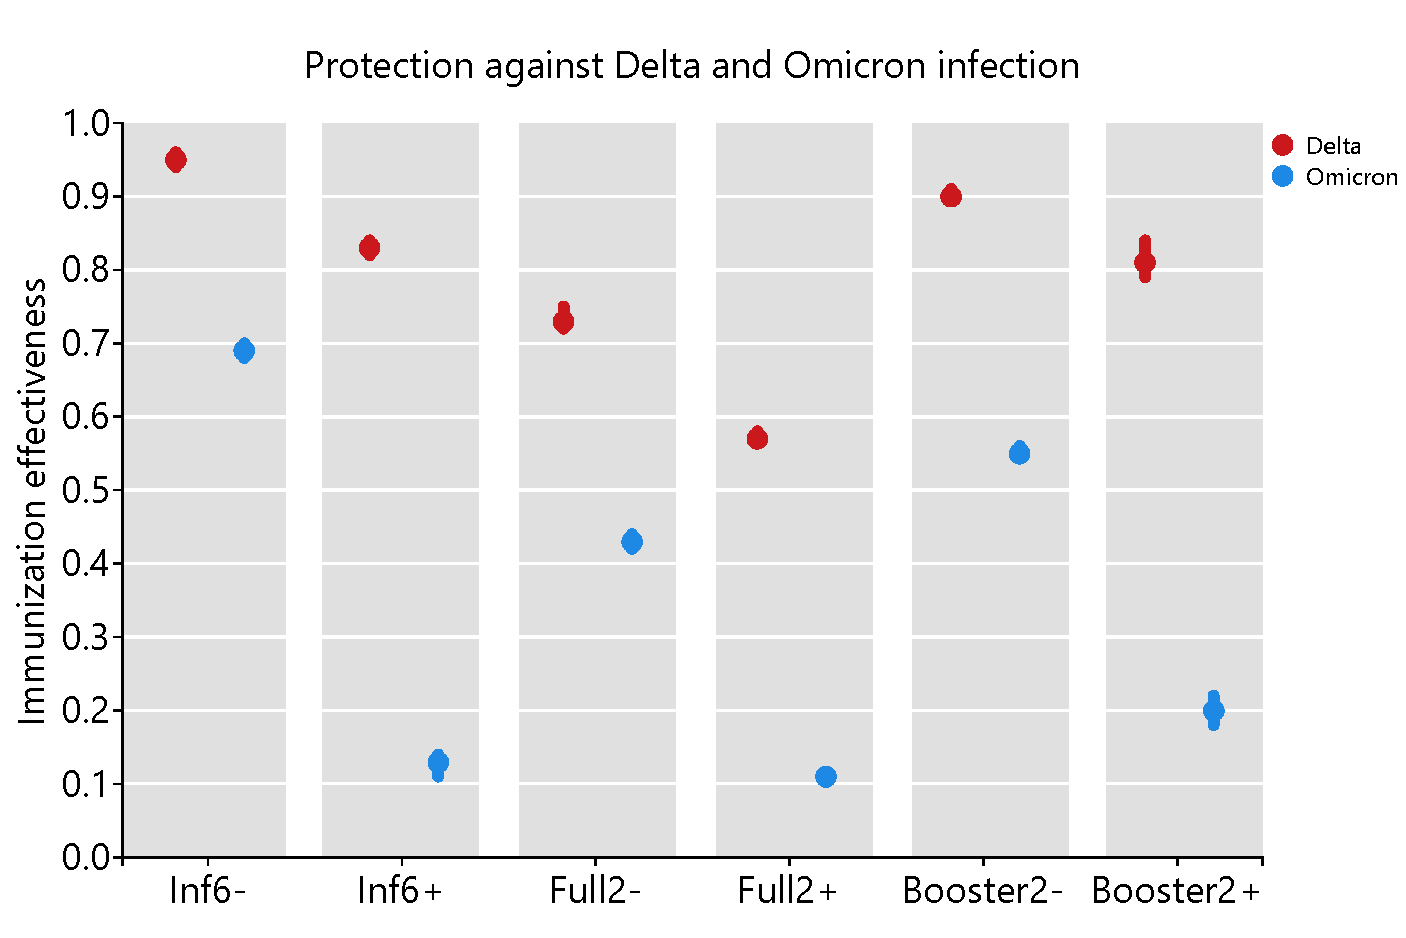
\includegraphics[width=0.9\textwidth]{fig2.pdf}
% \caption{Vaccine-acquired immunity against infection with respect to the delay from the full vaccine application, including the effect of a booster vaccine dose. %adjusted for sex and age.
% }
% \label{resfig2}
% \end{figure}

% A similar trend can be seen in the estimation of vaccine effectiveness against hospital admissions and deaths. For hospital admission, the vaccine effectiveness declined for Comirnaty from 90\% (95\% CI 89-91) at 0-2 months after dose 2 to 75\% (95\% CI 73-76) at 7-8 months, for Spikevax from 94\% (95\% CI 92-96) to 81\% (95\% CI 78-84), and for Vaxzevria from 87\% (95\% CI 81-91) at 0-2 months to 70\% (95\% CI 68-72) at 5-6 months  (Fig.\,\ref{resfig2} red curves, Table \ref{tab:vacc_hazard_ratios}). In the case of protection from death the model estimated for Comirnaty a decrease from 92\% (95\% CI 90-93) at 0-2 months to 83\% (95\% CI 81-86) at 7-8 months, from 96\% (95\% CI 91-98) to 88\% (95\% CI 82-92) for Spikevax within the first 8 months and from 93\% (95\% CI 77-98) to 82\% (95\% CI 78-85) for Vaxzevria within the first 6 months after application (Fig.\,\ref{resfig2} black curves, Table \ref{tab:vacc_hazard_ratios}). Janssen once again exhibits virtually no decline either in the protection against hospitalization starting from 68\% (95\% CI 60-75) at 2 months to 67\% (95\% CI 62-72) at 5-6 months, or deaths starting from 68\% (95\% CI 42-82) and reaching 68\% (95\% CI 53-78) at 5-6 months (Fig.\,\ref{resfig2}, Table \ref{tab:vacc_hazard_ratios}).


\section*{Discussion and Conclusions}
\label{sec4}

Our data support the existing evidence that the Omicron variant of SARS-CoV-2 evades to a significant extent both the post-vaccination and post-infection immunity \citep{mccallum2022,Dejnirattisai2022,Hoffmann2022,Cui2022,Cao2021}. The VEs of all the vaccines used in the Czech Republic are lower for Omicron compared to Delta. As we previously observed with Alpha and Delta \citep{Berec2021preprint}, the protection against infection by the Omicron variant wanes over time too. However, a booster vaccine dose provides robust and lasting or slowly waning protection against hospitalization, the need for oxygen therapy and intensive care. The combined post-infection and post-vaccination immunity is the most protective regardless of the exact sequence of events, suggesting that the best protective strategy before a coming wave is to vaccinate all individuals, whether previously vaccinated or with a previous covid-19 infection.

We are aware of the complicated interpretation of the hospitalization data for the Omicron wave, as the very high basic reproduction number $R_0$ of this variant \cite{nishiura2022relative} translated into the very high prevalence of infection in the population at the peak of the epidemic wave and a much higher proportion of hospitalized patients with covid-19 as a concomitant finding rather than the reason for admission. We therefore analysed separately the need for oxygen therapy and ICU admission as a more relevant measure of severe outcomes due to the Omicron infection.

Compared to the Delta variant, the protection provided by the post-infection or post-vaccination immunity is lower for the Omicron variant but at the same time the Omicron variant appears less severe than the Delta variant and the odds ratio for oxygen therapy or ICU admission are both approximately about one quarter compared to the Delta variant.

A common limitation of studies like ours is the fact that only a certain portion of infections is reported (ascertainment rate).  We believe this phenomenon does not affect significantly our estimates of vaccine effectiveness, assuming that the ascertainment rate is the same for the vaccinated and the unvaccinated alike and we have no evidence to the contrary. A difference in the ascertainment rate could also distort our estimates of the protection by the post-infection immunity; in particular, if there were undetected individuals with post-infection immunity in the control group, the infection risk of the population would be underestimated and, consequently, the protection by infection underestimated as well. Our results should be interpreted in terms of reported infections only. 

\acknow{%{\bf Data sharing.} 
Data reported in this study and used for the analyses are not public. De-identified individual-level data are available to the scientific community. Requests should be submitted to the Institute of Health Information and Statistics of the Czech Republic  ({\tt www.uzis.cz/index-en.php}), together with a short description of their analysis proposals, where they will be assessed based on relevance and scientific merit.
}


\showacknow{} % Display the acknowledgments section

% Bibliography
\bibliography{refs}


\end{document}


%\subsection*{Author Affiliations}

%Include department, institution, and complete address, with the ZIP/postal code, for each author. Use lower case letters to match authors with institutions, as shown in the example. PNAS strongly encourages authors to supply an \href{https://orcid.org/}{ORCID identifier} for each author. Individual authors must link their ORCID account to their PNAS account at \href{http://www.pnascentral.org/}{www.pnascentral.org}. For proper authentication, authors must provide their ORCID at submission and are not permitted to add ORCIDs on proofs.

%\subsection*{Submitting Manuscripts}

%All authors must submit their articles at \href{http://www.pnascentral.org/cgi-bin/main.plex}{PNAScentral}. If you are using Overleaf to write your article, you can use the ``Submit to PNAS'' option in the top bar of the editor window. 

%\subsection*{Format}

%Many authors find it useful to organize their manuscripts with the following order of sections;  title, author line and affiliations, keywords, abstract, significance statement, introduction, results, discussion, materials and methods, acknowledgments, and references. Other orders and headings are permitted.

%\subsection*{Manuscript Length}

%A standard 6-page article is approximately 4,000 words, 50 references, and 4 medium-size graphical elements (i.e., figures and tables). The preferred length of articles remains at 6 pages, but PNAS will allow articles up to a maximum of 12 pages.

%\subsection*{References}

%References should be cited in numerical order as they appear in text; this will be done automatically via bibtex, e.g. \cite{belkin2002using} and \cite{berard1994embedding,coifman2005geometric}. All references cited in the main text should be included in the main manuscript file.

%\subsection*{Data Archival}

%PNAS must be able to archive the data essential to a published article. Where such archiving is not possible, deposition of data in public databases, such as GenBank, ArrayExpress, Protein Data Bank, Unidata, and others outlined in the \href{https://www.pnas.org/page/authors/journal-policies#xi}{Information for Authors}, is acceptable.

%\subsection*{Language-Editing Services}
%Prior to submission, authors who believe their manuscripts would benefit from professional editing are encouraged to use a language-editing service (see list at www.pnas.org/page/authors/language-editing). PNAS does not take responsibility for or endorse these services, and their use has no bearing on acceptance of a manuscript for publication. 

%\begin{figure}%[tbhp]
%\centering
%\includegraphics[width=.8\linewidth]{frog}
%\caption{Placeholder image of a frog with a long example legend to show justification setting.}
%\label{fig:frog}
%\end{figure}


%\begin{SCfigure*}[\sidecaptionrelwidth][t]
%\centering
%\includegraphics[width=11.4cm,height=11.4cm]{frog}
%\caption{This legend would be placed at the side of the figure, rather than below it.}\label{fig:side}
%\end{SCfigure*}

%\subsection*{Digital Figures}

%EPS, high-resolution PDF, and PowerPoint are preferred formats for figures that will be used in the main manuscript. Authors may submit PRC or U3D files for 3D images; these must be accompanied by 2D representations in TIFF, EPS, or high-resolution PDF format. Color images must be in RGB (red, green, blue) mode. Include the font files for any text.

%Images must be provided at final size, preferably 1 column width (8.7cm). Figures wider than 1 column should be sized to 11.4cm or 17.8cm wide. Numbers, letters, and symbols should be no smaller than 6 points (2mm) and no larger than 12 points (6mm) after reduction and must be consistent. 

%Figures and tables should be labelled and referenced in the standard way using the \verb|\label{}| and \verb|\ref{}| commands.

%Figure \ref{fig:frog} shows an example of how to insert a column-wide figure. To insert a figure wider than one column, please use the \verb|\begin{figure*}...\end{figure*}| environment. Figures wider than one column should be sized to 11.4 cm or 17.8 cm wide. Use \verb|\begin{SCfigure*}...\end{SCfigure*}| for a wide figure with side legends.

%\subsection*{Tables}
%Tables should be included in the main manuscript file and should not be uploaded separately.

%\subsection*{Single column equations}

%Authors may use 1- or 2-column equations in their article, according to their preference.

%To allow an equation to span both columns, use the \verb|\begin{figure*}...\end{figure*}| environment mentioned above for figures.

%Note that the use of the \verb|widetext| environment for equations is not recommended, and should not be used. 

%\begin{figure*}[bt!]
%\begin{align*}
%(x+y)^3&=(x+y)(x+y)^2\\
       %&=(x+y)(x^2+2xy+y^2) \numberthis \label{eqn:example} \\
       %&=x^3+3x^2y+3xy^3+x^3. 
%\end{align*}
%\end{figure*}


%\begin{table}%[tbhp]
%\centering
%\caption{Comparison of the fitted potential energy surfaces and ab initio benchmark electronic energy calculations}
%\begin{tabular}{lrrr}
%Species & CBS & CV & G3 \\
%\midrule
%1. Acetaldehyde & 0.0 & 0.0 & 0.0 \\
%2. Vinyl alcohol & 9.1 & 9.6 & 13.5 \\
%3. Hydroxyethylidene & 50.8 & 51.2 & 54.0\\
%\bottomrule
%\end{tabular}

%\addtabletext{nomenclature for the TSs refers %to the numbered species in the table.}
%\end{table}

%\subsection*{Supporting Information Appendix (SI)}

%Authors should submit SI as a single separate SI Appendix PDF file, combining all text, figures, tables, movie legends, and SI references. SI will be published as provided by the authors; it will not be edited or composed. Additional details can be found in the \href{https://www.pnas.org/authors/submitting-your-manuscript#manuscript-formatting-guidelines}{PNAS Author Center}. The PNAS Overleaf SI template can be found \href{https://www.overleaf.com/latex/templates/pnas-template-for-supplementary-information/wqfsfqwyjtsd}{here}. Refer to the SI Appendix in the manuscript at an appropriate point in the text. Number supporting figures and tables starting with S1, S2, etc.

%Authors who place detailed materials and methods in an SI Appendix must provide sufficient detail in the main text methods to enable a reader to follow the logic of the procedures and results and also must reference the SI methods. If a paper is fundamentally a study of a new method or technique, then the methods must be described completely in the main text.

%\subsubsection*{SI Datasets} 

%Supply .xlsx, .csv, .txt, .rtf, or .pdf files. This file type will be published in raw format and will not be edited or composed.



%\subsubsection*{3D Figures}

%Supply a composable U3D or PRC file so that it may be edited and composed. Authors may submit a PDF file but please note it will be published in raw format and will not be edited or composed.


%\matmethods{Please describe your materials and methods here. This can be more than one paragraph, and may contain subsections and equations as required. 

%\subsection*{Subsection for Method}
%Example text for subsection.
%}

%\showmatmethods{} % Display the Materials and Methods section

%\acknow{Please include your acknowledgments here, set in a single paragraph. Please do not include any acknowledgments in the Supporting Information, or anywhere else in the manuscript.}
